\section{Summary}
In this chapter we will use the textural developed in previous chapters 
to create a change detection algorithm (CDA). The CDA will be assessed
using the CARABAS-II image dataset, which is a set of images acquired by a Very High Frequency (VHF) Ultra Wideband (UWB) SAR system.
The CDA is based on the UNET convolutional neural network (CNN) architecture and will use the 
textural information as additional inputs for image classification.
It will be demonstrated that the 
use of textural information can improve the overall performance of the algorithm
in terms of probability of detection and false alarm rate. 

\section{Introduction}
As previously mentioned, SAR has several applications, such as, topology, oceonography, geology, environment monitoring, among others.
The SAR can operate in two modes: single-pass acquisition and multi-pass acquisition. In the first it is captured only one picture of the 
monitored area, while in the latter there can be multiple acquisitions of the same area. 
When dealing with multi-temporal acquisitions, we can either assess the information contained in the entire time frame or focus in detecting changes between the acquisitions. 
When the latter is the focus, change detection algorithms (CDA) are traditionally used to identify the relevant changes \cite{Carabas, Ricardo}.

Generally, CDA's priority is the percentage of true positives with a lower regard for percentage of false positives. 
Those can however be relevant in many applications such as detecting hidden objects over a large area, 
where a small number of false positives is vital in the quality of the final data for operation application - which is the main concern of this work. 
While trying to develop a CDA for this work, it was kept in mind that the CDA developed would have to provide a high percentage of true positives while trying to minimize
the amount of false positives.

The traditional method for creating CDAs was to base the decisor on standard statistical theory, e.g, traditional hypothesis testing criterion methods,
such as 
generalized likelihood ratio test \cite{GLRT1,GLRT2,GLRT3}, 
maximum a posteriori criterion \cite{Book_Kay},
Bayesian theory approaches \cite{Bayes1, Bayes2},
or likelihood ratio test \cite{LRT1,LRT2,LRT3}. Even though these methods, most of the time, perform adequately in terms of probability of detection, but
most of them show poor performance in terms of false alarm rate \cite{Carabas,Ricardo,LucasRamos,Chris}. Those methods also have a few drawbacks, such as: depending on
additional preprocessing of the images throughout morphological operations (erosion and dilation filters have to normally be used) and depend on calibration of the algorithm
for the statistical analysis to work.

By trying to overcome the limitations of traditional statistical based CDAs, machine learning algorithms became popular in the last few years \cite{Vinholi, Campos} since they
have the capability to perform better than statistical based CDAs and don't have the usual drawbacks that those methods present. There are two kinds of machine learning algorithms: supervised and unsupervised
algorithms. Supervised algorithms are the ones that have a  classification reference to help guide the learning step, while unsupervised algorithms are the ones that do not have this classification reference - 
on this work we focused only in supervised algorithms. As it was mentioned, it is important to know what is the parameter of interest to quantify the quality of the algorithm, e.g., we can assess performance
based on number of true positives, true negatives, false positives and false negatives \cite{PefMe} - for this part of the work, the parameters of interest are number of true positives and number of false negatives.

Among supervised machine learning algorithms there are multiple algorithms that can be chosen to solve the problem, such as: Neural Networks, Naive Bayes, Linear Regression, Kernel Ridge Regression, Support Vector Machine, Decision Trees, Random Forest \cite{PefMe}.
For this work it was chosen to use a neural network based algorithm for the CDA. There are multiple types of neural networks, e.g., perceptron, Feed Forward Neural Network, Multilayer Perceptron, Recurrent Neural Network, Long Short-Term Memory Neural Network, convolutional
neural network, among others \cite{PefMe}. It was chosen to use a convolutional neural network, specifically a UNET convolutional neural network \cite{Unet}, for solving the target detection problem, since convolutional neural network have shown
excellent results for computer vision problems. In \cite{Kevin} it was used a similar approach to detect change in SAR images, although in \cite{Kevin} the SAR images were acquired in a much higher frequency. 
  
The UNET CNN will not only have the SAR acquisitions as input for the target detection, but will also have textural information that will be extracted according to the methods explained in 
chapter 3. 
In \cite{Rodrigo} it was already shown that additional textural information can provide valuable information to improve classification results. It is important to mention that since CNN use convolutions, which are linear filters, to achieve better classification results,
it would be redundant to use linear textural information as inputs to the UNET CNN.  When comparing the proposed technique with other algorithms on the same dataset, we show that the results show similar detection performance but presenting a significant false alarm rate improvement.

\begin{figure}[ht]
    \centering
    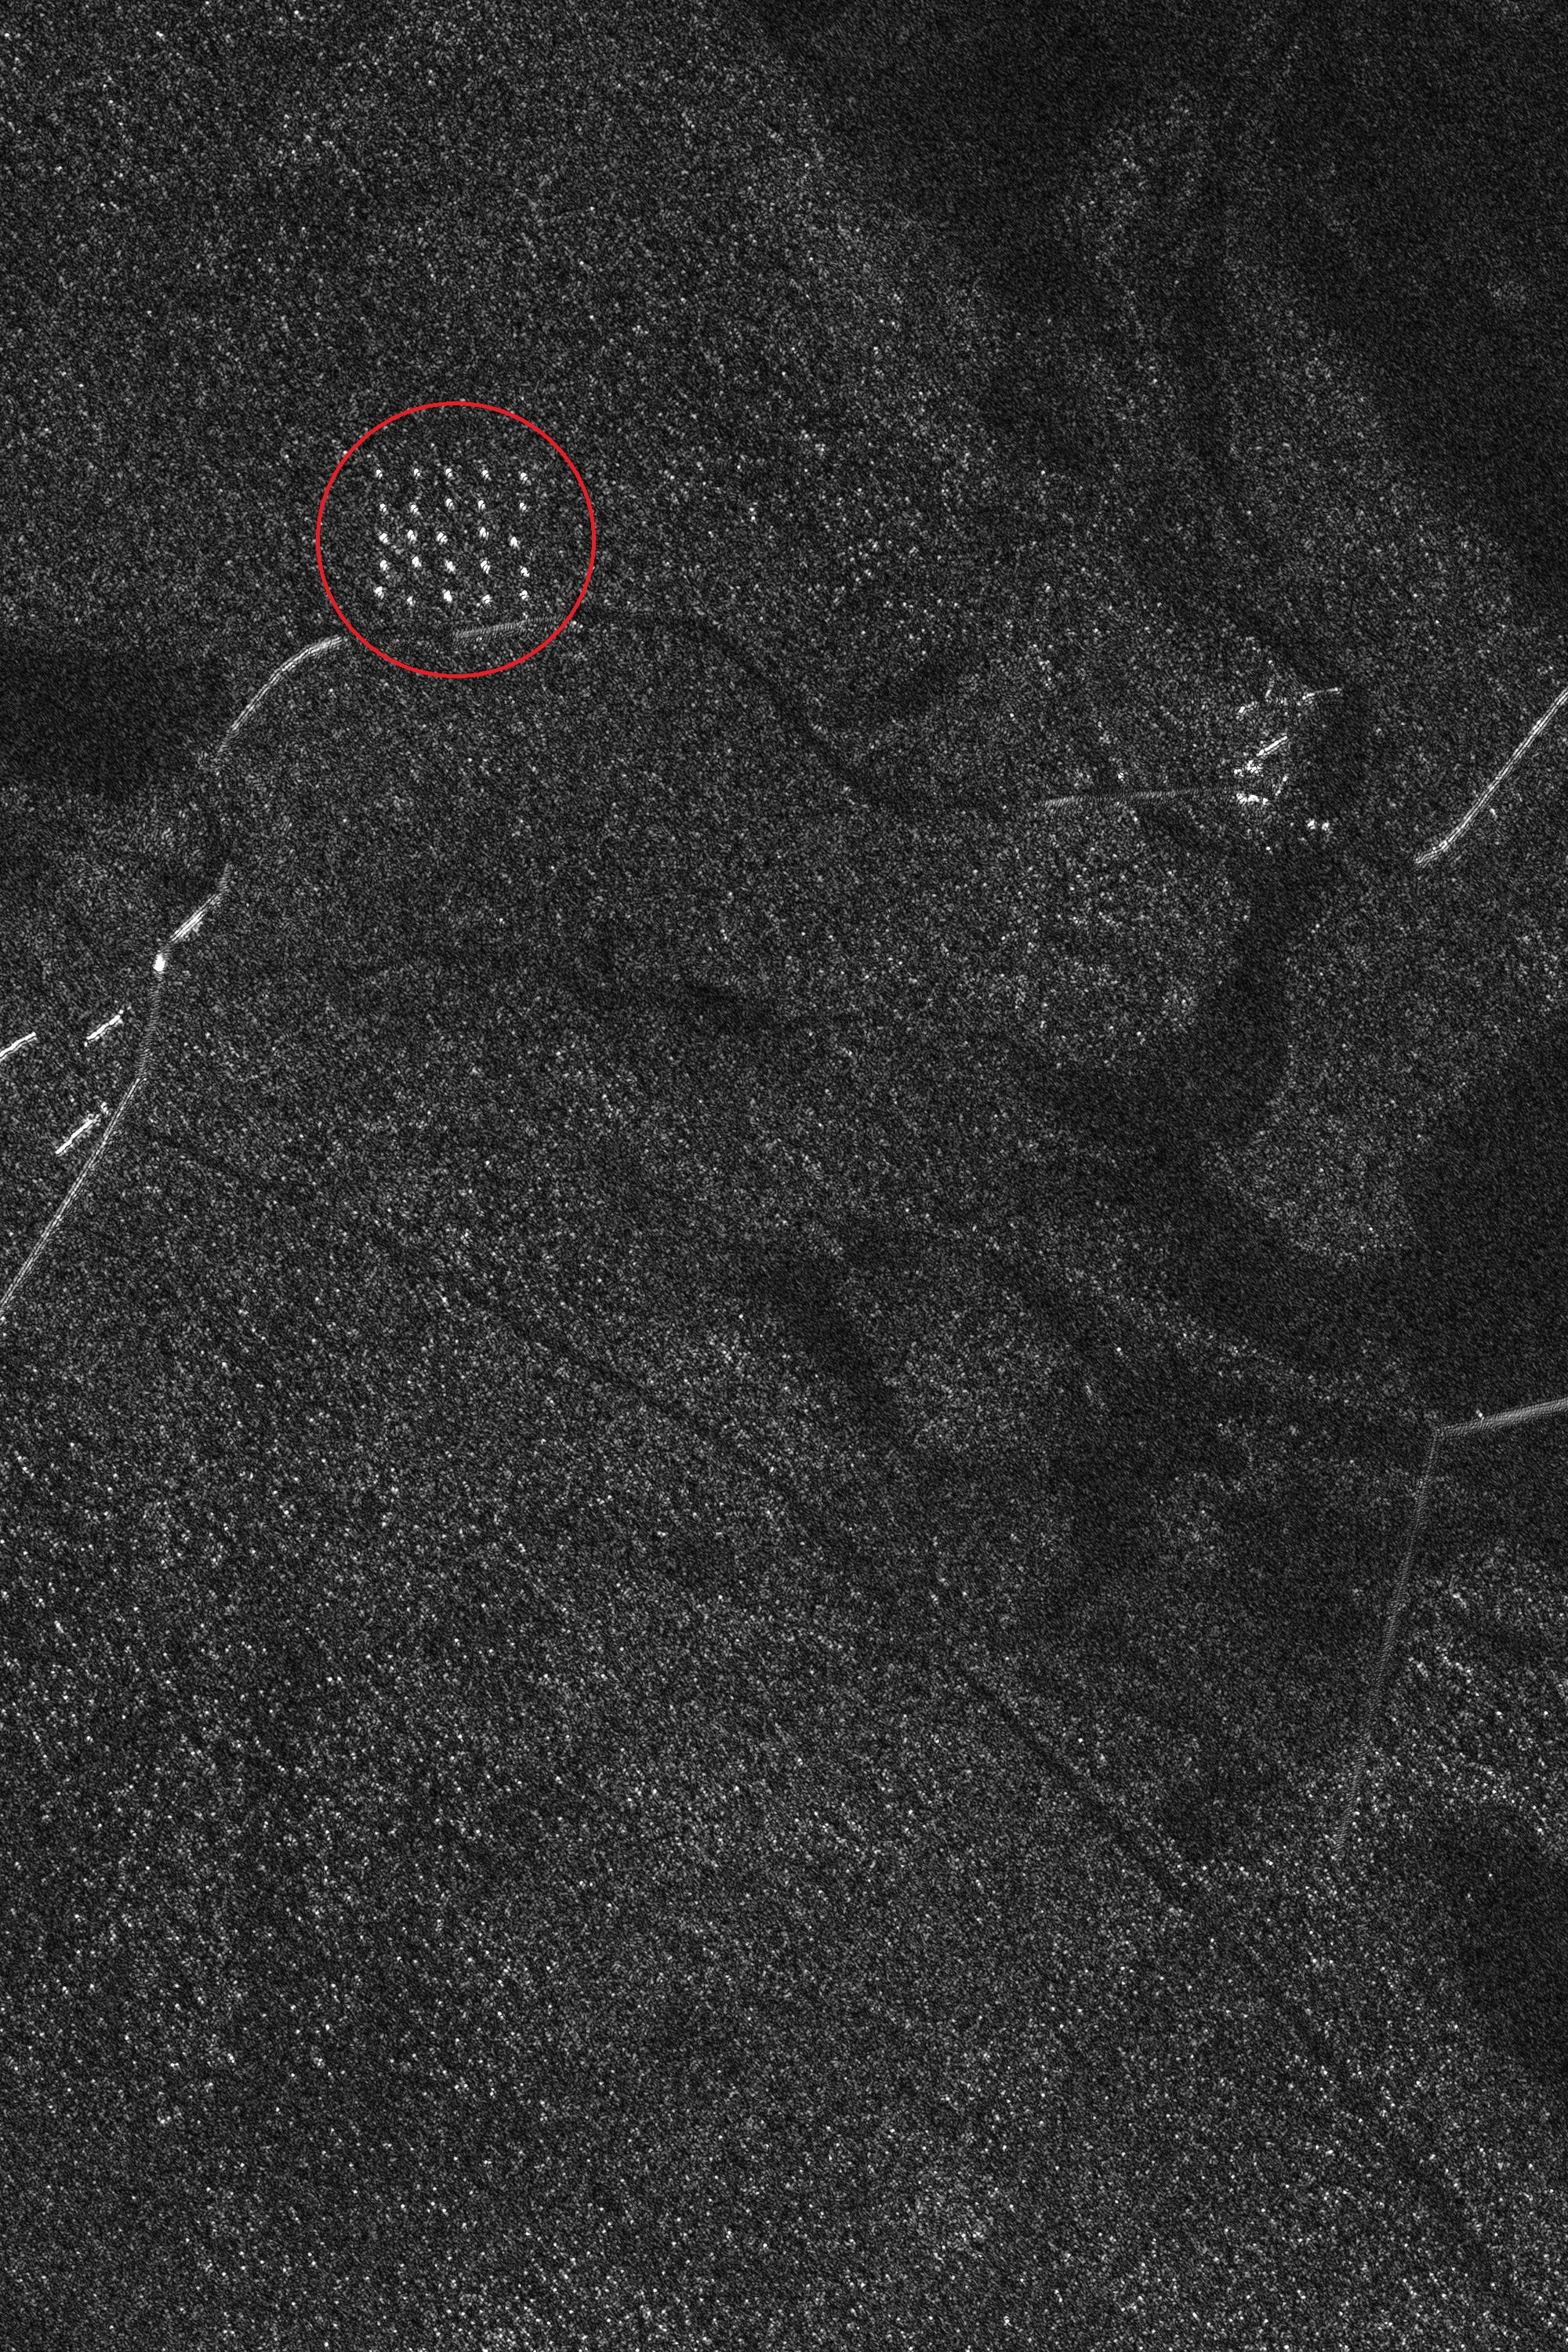
\includegraphics[width=0.45\linewidth]{Chapter7/exemplo_carabas.jpg}
    \caption{ Example of a SAR image acquired by the CARABAS-II system.
    The red circle shows the position of the cars hidden under a canopy of trees.}
    \label{fig:exemplo_carabas}
\end{figure}

\section{Relevant Textures for the Change Detection Algorithm}
As it was done in \cite{Rodrigo} we will use the method of Sum and Difference Histograms to compute the textures \cite{Sarker,Sarker2}, since they have been demonstrated to compute 
useful textures to be used as additional information for machine learning algorithms and it is a texture computation method that can run in linear time. We will again give a brief overview of the method.

For a given SAR image, we consider the random variable $u_{[x, y]}$ to be the absolute value of the backscatter value received by the antenna. The first step of the algorithm is to 
quantize the random variable $u$ to have $N_g$ discrete integer possible values (on this work $N_g$ was chosen to be 20). The second step is to obtain an estimate of the joint probability density function of the random v $[u_{[x,y]}, u_{[x+\delta x, y+\delta y]}]$ (where $\delta = (\delta x, \delta y)$ is the displacement vector 
chosen to compute the texture direction and distance),
which is a $N_g \times N_g$ matrix. According to \cite{ Unser}, it is possible to create an estimate of this Joint PDF in linear time by creating a random gaussian vector that has uncorrelated, therefore independent, random variables, and then computing the textures 
directly from the two linear independent variables. The new vector is $[s_{[x,y]}, d_{[x, y]}]$ and is obtained as follows:

\begin{equation}
    \begin{array}{ccc}
         s_{[x,y]} &=& u_{[x,y]} + u_{[x+\delta x, y+\delta y]} \\
         d_{[x,y]} &=& u_{[x,y]} - u_{[x+\delta x, y+\delta y]}
    \end{array}.
\end{equation} 

Since $s_{[x,y]}$ and $d_{[x,y]}$ are independent, it is possible to decompose the original Joint PDF as the product of two PDF as follows:
\begin{equation}
    \begin{array}{rrr}
       P(u_{[x,y]}=u_1, u_{[x+\delta x, y+\delta y]}=u_2) = \\ P(s_{[x,y]}=u_1+u_2, d_{[x,y]}=u_1-u_2) = \\
    P(s_{[x,y]}=u_1+u_2) \cdot P(d_{[x,y]} = u_1-u_2) 
    \end{array}
\end{equation}

By doing this it is now possible to compute the textures directly from the random variables $P_s$ and $P_d$. Notice that by doing this, the time 
complexity of the texture calculation was reduced from $O(N_g^2)$ to $O(2*N_g)$.

\begin{figure}[ht]
    \centering
    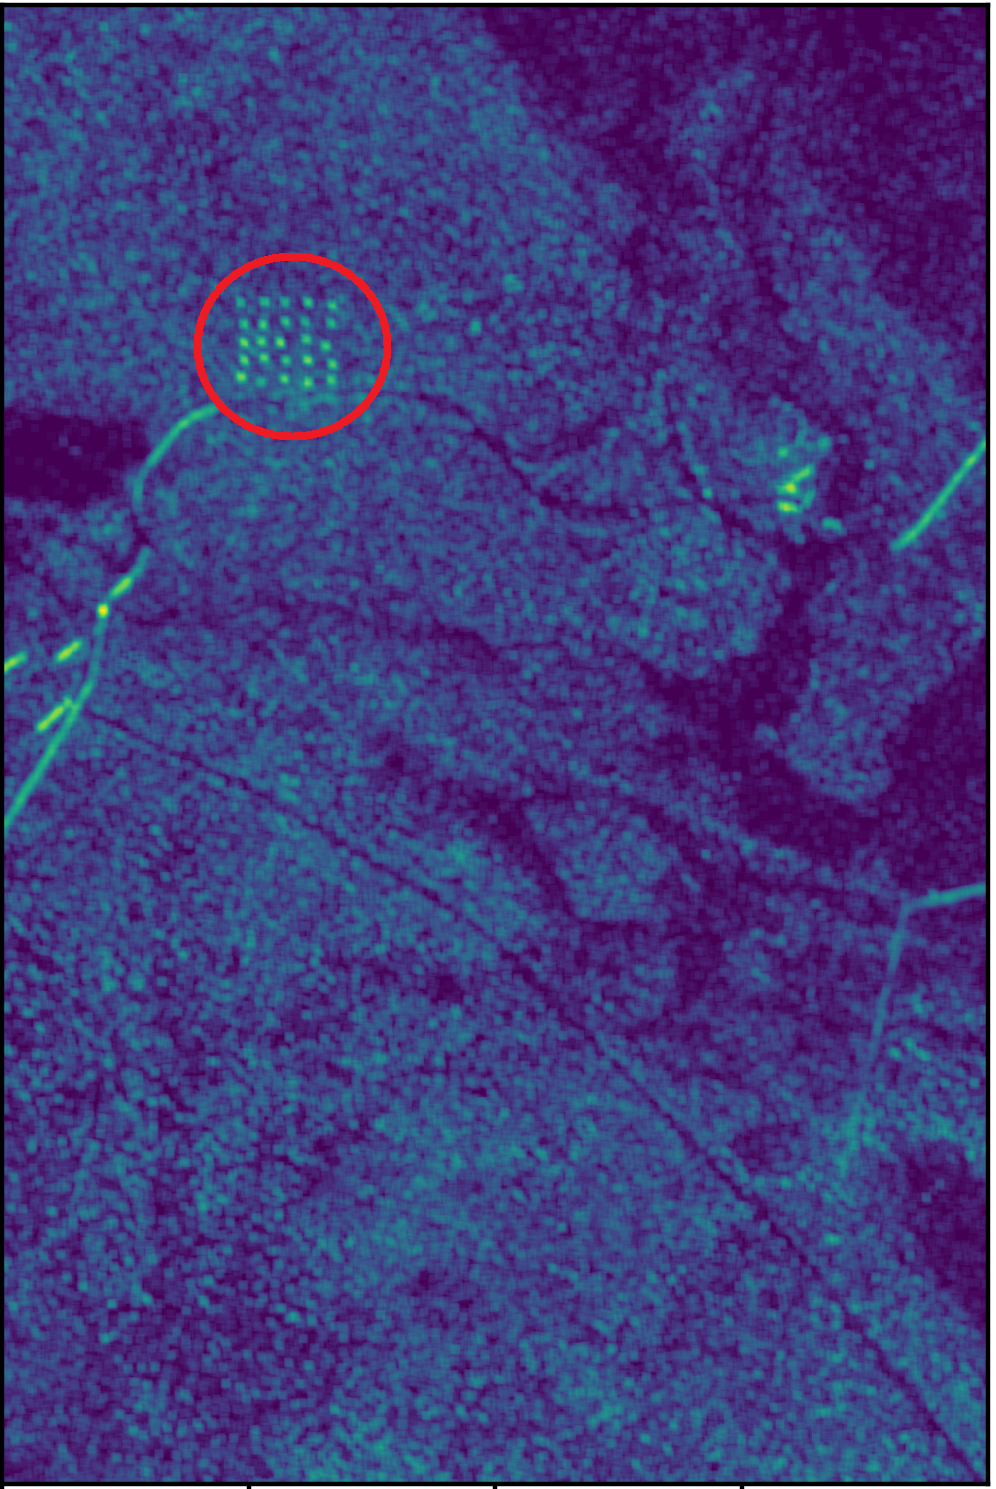
\includegraphics[width=0.45\linewidth]{Chapter7/entropy_examplepng.png}
    \caption{Entropy image. The red circle shows the position of the vehicles.}
    \label{fig:entropy_example}
\end{figure}

After obtaining the probability density functions $P(s_{[x,y]})$ and $P(d_{[x,y]})$, a set of textural information can be extracted as follows (for better readability, we define $P_s(i) = P(s[x,y] = i)$ and $P_d(j) = P(d[x,y] = j))$:
\begin{enumerate}
    \item Mean($\mu$): describes the mean value of the co-occurrences and is given by
    \begin{equation}
        \textrm{MEAN} = \frac{1}{2}\sum_{i=1}^{N_g}i\cdot P_s(i)
    \end{equation}
    
    \item Cluster prominence: describes the fourth moment of the random variables and is given by
    \begin{equation}
        \textrm{CLP} = \sum_{i=1}^{N_g}(i-2\mu)^4\cdot P_s(i)
    \end{equation}
    
    \item Cluster shade: describes the third moment of the random variables and is given by
    \begin{equation}
        \textrm{CLS} = \sum_{i=1}^{N_g}(i-2\mu)^3\cdot P_s(i)
    \end{equation}
    
    \item Contrast: measure the difference of intensities of co-occurrences in the image and is given by
    \begin{equation}
        \textrm{CON} = \sum_{j=\frac{-N_g}{2}}^{\frac{N_g}{2}}(j)^\cdot P_d(j)
    \end{equation}
    
    \item Correlation: describes the linear correlation of intensities of co-occurrences in the image and is given by
    \begin{equation}
        \textrm{COR} = \frac{1}{2}\sum_{i=1}^{N_g}(i-2\mu)^2\cdot P_s(i)-\frac{1}{2}\sum_{j=\frac{-N_g}{2}}^{\frac{N_g}{2}}(j)^\cdot P_d(j)
    \end{equation}
    
    \item Energy: describes the energy of the received signal and is given by
    \begin{equation}
        \textrm{ENE} = \sum_{i=1}^{N_g}P_s(i)^2\cdot \sum_{j=\frac{-N_g}{2}}^{\frac{N_g}{2}} P_d(j)^2
    \end{equation}
    
    \item Entropy: describes the uncertainty of the co-occurrence matrix and is given by
    \begin{equation}
        \textrm{ENT} = -\sum_{i=1}^{N_g}P_s(i)\log(P_s(i)) - \sum_{j=\frac{-N_g}{2}}^{\frac{N_g}{2}} P_d(j)\log(P_d(j))
    \end{equation}
    
    \item Homogeneity: describes the degree of similarity between images and is given by
    \begin{equation}
        \textrm{HOM} = - \sum_{j=\frac{-N_g}{2}}^{\frac{N_g}{2}} \frac{P_d(j)}{1+j^2}
    \end{equation}
    
    \item Variance: describes the degree of dispersion of intensities between two images and is given by
    \begin{equation}
        \textrm{VAR} = \frac{1}{2} \sum_{i=1}^{N_g}(i-2\mu)^2 P_s(i) + 
         \frac{1}{2}\sum_{j=\frac{-N_g}{2}}^{\frac{N_g}{2}} j^2 P_d(j)
    \end{equation}
\end{enumerate}

There are multiple textures that can be chosen as additional inputs for the UNET CNN. One have to keep in mind, that, for every texture that it is used as additional information, 
the time computation for the training and validation of the UNET will be also increased, so it is vital to keep in mind the trade-off between computation time and improvement of classification results.

For this work it was chosen to use the Entropy and Variance images textures as additional information. The original picture and the texture pictures can be seen in \figref{fig:exemplo_carabas}, \figref{fig:entropy_example} and \figref{fig:variance_example}.



\begin{figure}[ht]
    \centering
    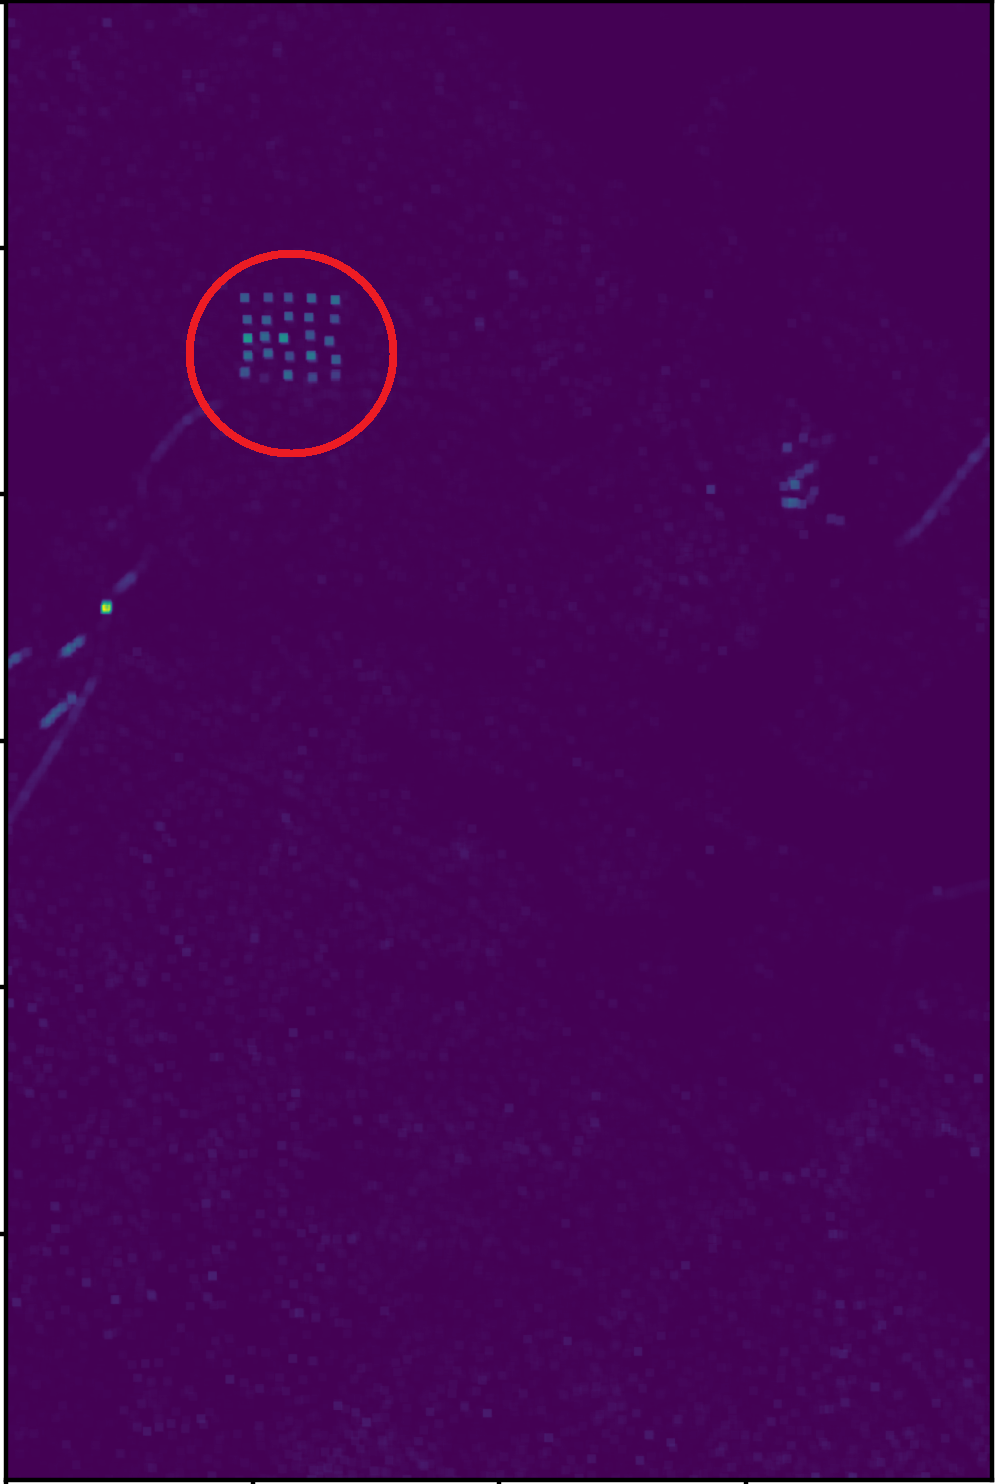
\includegraphics[width=0.45\linewidth]{Chapter7/variance_exemplo.png}
    \caption{Variance image. The red circle shows the position of the vehicles.}
    \label{fig:variance_example}
\end{figure}

\section{UNET Based Algorithm for Target Change Detection}
The UNET is a convolutional neural network that was developed in the Computer Science department of the University of Freiburg for the purpose of performing image segmentation for
biomedical pictures \cite{Unet}. It became popular because it was able to perform precise segmentations with little time (segmentation of a 512x512 image takes less than a second using a modern GPU).
Convolutional Neural networks normally work by performing a series of convolutions and pooling filters that decrease the size of the image, while the UNET works by also 
supplementing this usual operation pipeline with a series of successive layers in which the pooling operations are replaced by upsampling operators, therefore increasing the resolution of the output.
The final goal is that a usual successive convolutional layer learn to create an output based on this information. 

It is important to remind that an important aspect of the UNET is that there is a large number of feature channels responsible for the upsampling step, which ensures that the UNET propagates information
to the higher resolution layers. After the expansive path is performed, it is combined with the usual pooling operations, creating a contractive path, which makes the UNET shows a u-shaped architecture. 
It is important also to mention that in the borders of the image, the UNET will extrapolate by mirroring the information to predict the pixels in the area. 
\figref{fig:unet_architecture} depicts the architecture of the UNET and it's u-shape.

\begin{figure}[ht]
    \centering
    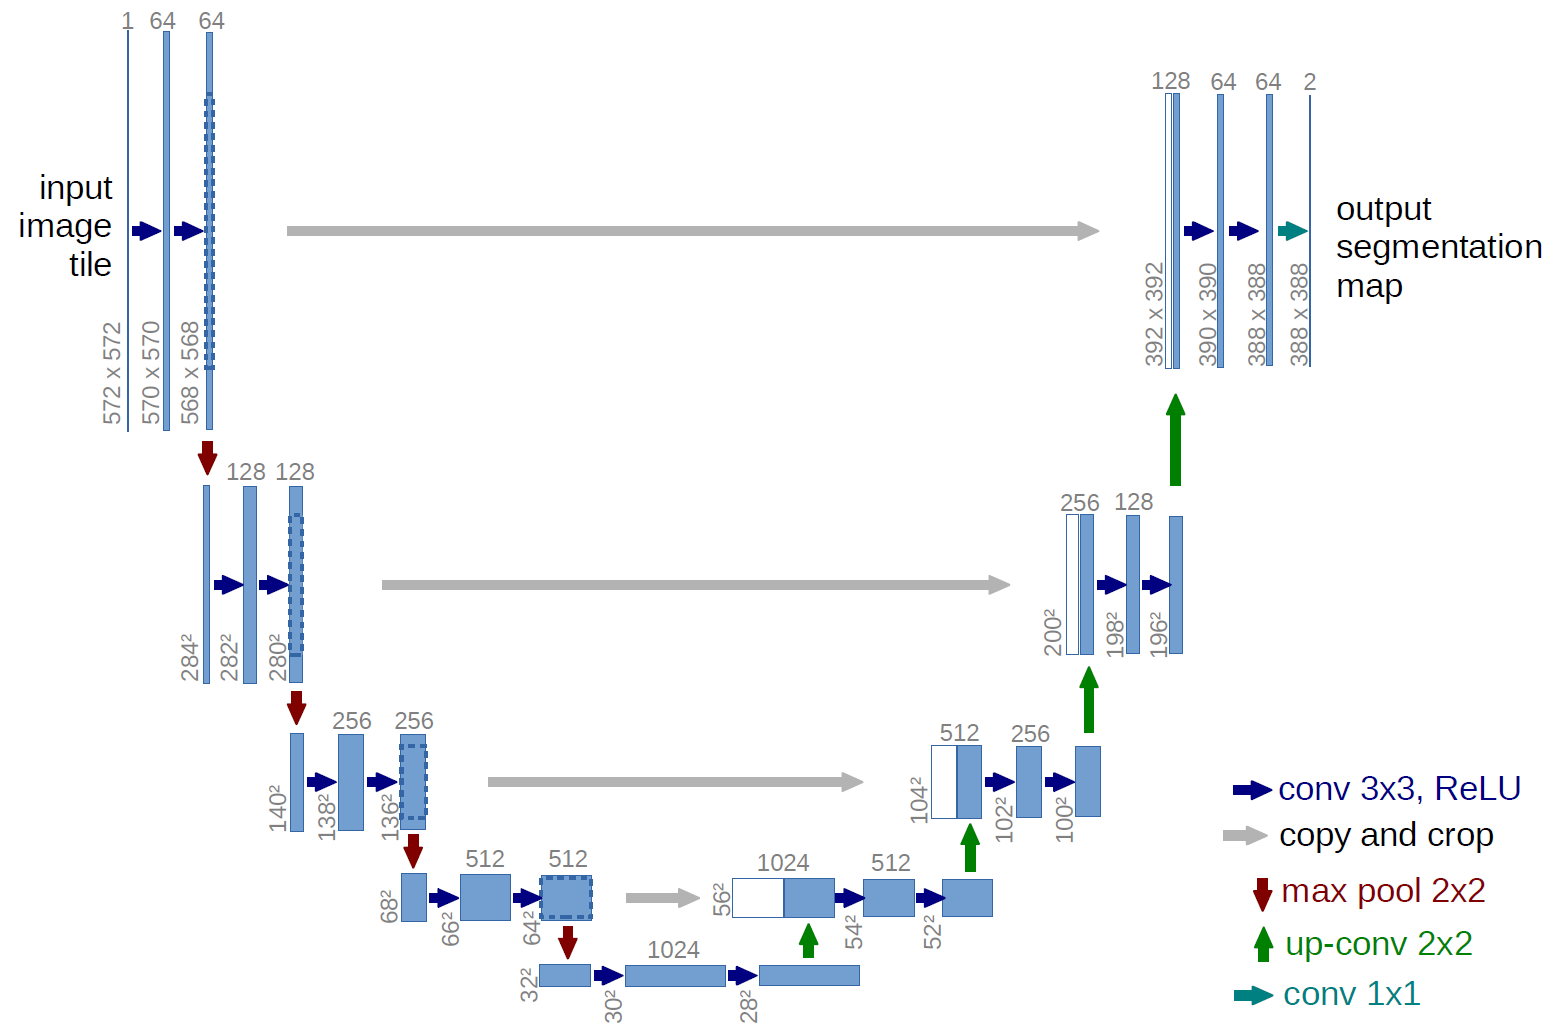
\includegraphics[width=0.7\linewidth]{Chapter7/unet_architecture.png}
    \caption{UNET architecture.}
    \label{fig:unet_architecture}
\end{figure}

The proposed CDA is based on this UNET architecture and has two phases: the training phase and the inference phase.

\textit{A. Training Phase}
\newline
In this phase the model is treated like a regular supervised machine learning model. The given UNET architecture is trained in a supervised manner with the reference map
to be able to perform semantic image segmentation. 
\newline
\textit{B. Inference Phase}
\newline
This phase is based on the Change Detection algorithm proposed by \cite{Kevin}. This algorithm was based on modifying the original UNET two accept two images for the purpose of change detection.
The original algorithm has 5 feature maps created by the convolutions that were generated and saved for the first image. After that, when the second image is used as input, a Difference Image (DI) is
created at each of the 5 levels using the feature maps of the first and second image.
The DI is created by taking the absolute value of the difference between the feature maps, and setting the difference to be zero if the difference value does not surpass a threshold value (which was found empirically), and setting it to 
the value of the second image if it surpasses the threshold value. Intuitivelly this step works by setting it to zero all pixels that did not change sufficient (according to a threshold value). After that, the DI is semantically segmentated, rendering a visual 
interpretation of the collective changes that happened. A visual representation of this algorithm is show in \figref{fig:kevin_algorithm}.

\begin{figure}[ht]
    \centering
    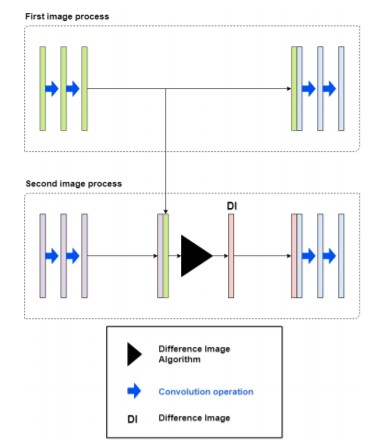
\includegraphics{Chapter7/kevin_algorithm.jpg}
    \caption{Inference Phase for the corresponding DI.}
    \label{fig:kevin_algorithm}
\end{figure}

The CDA of this work is inspired by the algorithm explained above. Since the textures provide additional information, it would be very 
hard to empirically achieve the values for the threshold of each layer (in our case it would be a vector instead of a scalar), so it was decided to perform the difference image
just for first input layer of the UNET.
We used the textures of Entropy and Variance, which was combined with the original image to create a three-channel tensor which was fed, and trained, on the UNET.

\begin{figure}[ht]
    \centering
    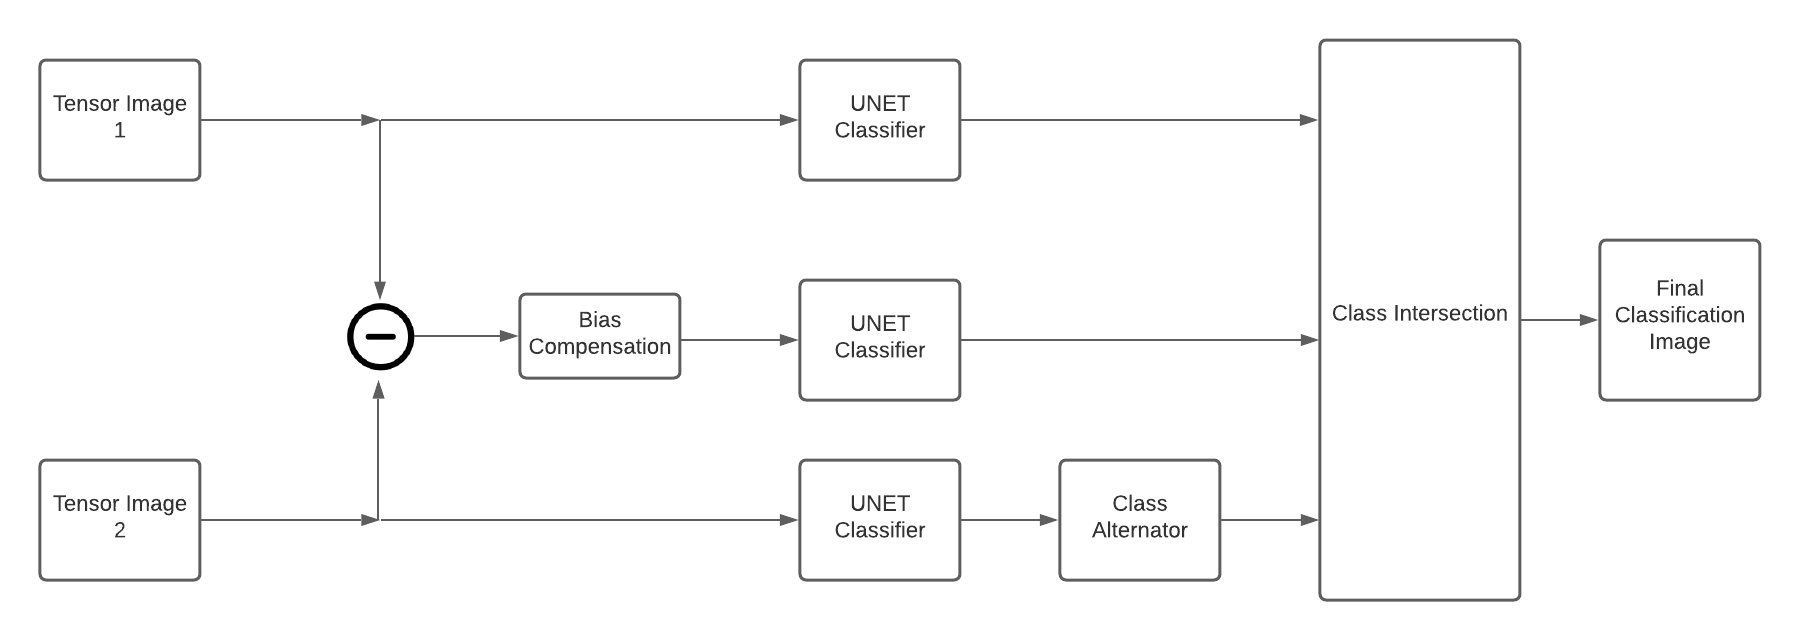
\includegraphics[width=\linewidth]{Chapter7/diagrama.png}
    \caption{ Diagram of the proposed algorithm.}
    \label{fig:diagrama}
\end{figure}

After creating the 24 image tensors, the dataset was divided into 12 tensors for training and 12 tensors for validation purposes. 
After the training was performed this trained UNET was used as part of the CDA.
The proposed CDA has 4 steps, and works as follows:
\begin{enumerate}
    \item Feed the first tensor as a input to the UNET and get the classification
    \item Feed the second tensor as input to the UNET, and after that alternate the classes from the final image (switch all car classification pixels by forest classification pixels and vice-versa)
    \item Take the absolute value of the difference of the tensors, perform a bias correction (the value for the bias correction was adjusted manually). After that feed this tensor as input to the UNET.
    \item Get the three classifications obtained prior and take the intersection of all classes (in order to a pixel to be classified as a car in the final image, it has to be a car in all of the three images at the same time)
\end{enumerate}

Item 2 was added to the algorithm simply to made it more robust against false errors. By adding another necessary step to identify the change as a target change difference
we decrease the probability of false detection, but at the same time it will also decrease the overall probability of true detection for the algorithm. 

After the final image is created by the CDA, a threshold filter selection was performed to eliminate noise classification from the image - we considered only sets of pixels which had 100 or more connected components.

In \figref{fig:diagrama} the proposed algorithm is represented visually.



\begin{table}[ht]
    \centering
    \begin{tabular}{c|c||c|c|c|c}
         \vtop{\hbox{\strut Monitored}\hbox{\strut Image}} &
         \vtop{\hbox{\strut Reference}\hbox{\strut Image}}
         &\vtop{\hbox{\strut \vtop{\hbox{\strut Detected}\hbox{\strut Targets}}}\hbox{\strut \vtop{\hbox{\strut (with}\hbox{\strut texture)}}}}
         &\vtop{\hbox{\strut \vtop{\hbox{\strut False}\hbox{\strut Alarms}}}\hbox{\strut \vtop{\hbox{\strut (with}\hbox{\strut texture)}}}}
         &\vtop{\hbox{\strut \vtop{\hbox{\strut Detected}\hbox{\strut Targets}}}\hbox{\strut \vtop{\hbox{\strut (without}\hbox{\strut texture)}}}}
         &\vtop{\hbox{\strut \vtop{\hbox{\strut False}\hbox{\strut Alarms}}}\hbox{\strut \vtop{\hbox{\strut (without}\hbox{\strut texture)}}}}
         \\
         \hline
         2\_1&3\_1&25&0&25&0\\
         3\_1&4\_1&23&1&21&1\\
         4\_1&5\_1&25&0&25&0\\
         5\_1&2\_1&25&0&25&0\\
         \hline
         2\_2&4\_2&25&0&25&0\\
         3\_2&5\_2&25&0&23&1\\
         4\_2&2\_2&23&0&25&0\\
         5\_2&3\_2&22&0&24&0\\
         \hline
         2\_3&5\_3&25&0&25&0\\
         3\_3&2\_3&22&1&21&1\\
         4\_3&3\_3&25&1&25&1\\
         5\_3&4\_3&25&0&25&0\\
         \hline
         2\_4&3\_4&25&0&25&0\\
         3\_4&4\_4&24&0&23&1\\
         4\_4&5\_4&25&0&25&0\\
         5\_4&2\_4&24&0&25&0\\
         \hline
         2\_5&4\_5&25&0&25&0\\
         3\_5&5\_5&24&0&21&2\\
         4\_5&2\_5&25&0&25&0\\
         5\_5&3\_5&23&0&24&0\\
         \hline
         2\_6&5\_6&25&0&25&0\\
         3\_6&2\_6&23&1&25&0\\
         4\_6&3\_6&24&0&25&0\\
         5\_6&4\_6&25&1&25&0\\
    \end{tabular}
    \caption{Results of CDA in terms of detected targets and false alarm rate  for the same image pairs considered in (\cite{Carabas}). It is also presented  the results when textural information is either used or not used as input of the proposed algorithm.}
    \label{tab:my_table}
\end{table}

\section{Results}

As previously mentioned, the dataset of 24 images was divided into two parts: 12 images used for training the UNET and 12 images used for validation of the UNET training.
After that 24 images pairs were selected to assess the quality of the change detection algorithm. The 24 pairs follow the standard selection that are used to validate CDAs in the CARABAS dataset, as done in \cite{Carabas,Ricardo,LucasRamos}.

The results are presented in Table \ref{tab:my_table}, where each image M\_P was labelled in terms of Mission number (M) and flight pass (P). The compared images have different mission numbers, but the same flight pass heading.
In Table \ref{tab:my_table} it is presented the results for the CDA algorithm using only the original image -in order to assess the quality of the CDA-  and it is also presented the result using the textural information combined with the original image -
in order to assess the quality improvement due to the additional textural information.

The quality of the algorithm can be measured in terms of probability of detection and False Alarm Rate (FAR). The proposed algorithm achieved a Probability of detection of 97\% and a False Alarm Rate of 0.034${/} km^2$, while the original algorithm proposed in the CARABAS
challenge paper achieved a probability of detection of 97\% and a FAR of  $0.67{/} km^2$. Other recent algorithms, such as the one presented in \cite{Ricardo} achieved a probability of detection of 97\% and a FAR of $0.28{/} km^2$ and \cite{Vinholi} achieved a 
probability of detection of 99\% and a FAR of $0.0833{/} km^2$. 

\section{Conclusion}
The Change Detection Algorithm proposed yielded a probability of detection similar to the usual state-of-the-art algorithms existent - it had a probability of detection of 97\% - 
but showed great improvements in terms of False Alarm Rate, reducing the probability of false alarm more than ten times, when compared to usual statistical change detection algorithms, and 
and reducing the probability of false alarm almost three times when compared to usual Convolutional Neural Network based machine learning algorithms.